\documentclass[10pt,journal,compsoc]{IEEEtran}

\usepackage{cite}
\usepackage{amsmath,amssymb,amsfonts}
\usepackage{algorithmic}
\usepackage{graphicx}
\usepackage{textcomp}
\usepackage{xcolor}
\usepackage{booktabs}
\usepackage{multirow}
\usepackage{url}
\usepackage{microtype}
\graphicspath{{../figures/}{figures/}{../figures/figures/}}

\begin{document}

\title{What Do LLMs Say That Human Facilitators Don't? A Computational Behavioral Analysis of AI vs.\ Human Collaborative Design Meeting Facilitation}

\author{Mohammed Azeez Khan, Aaron D'Souza, Ashutosh Mishra, and Amar Kumar Behera%
\IEEEcompsocitemizethanks{
\IEEEcompsocthanksitem M. A. Khan is with the Department of Computer Science and Engineering, National Institute of Technology Warangal, Warangal, India. E-mail: mohammedazeezkhan@student.nitw.ac.in.
\IEEEcompsocthanksitem A. D'Souza and A. Mishra are with the Department of Electronics and Communication Engineering, National Institute of Technology Warangal, Warangal, India.
\IEEEcompsocthanksitem A. K. Behera is with the Department of Design, Indian Institute of Technology Kanpur, Kanpur, India.
}}

\markboth{arXiv Preprint}{Khan \emph{et al.}: Computational Behavioral Analysis of AI vs.\ Human Design Facilitation}

\IEEEtitleabstractindextext{%
\begin{abstract}
Artificial intelligence is increasingly explored for assisting collaborative design meeting facilitation, yet empirical comparisons between large language models (LLMs) and human facilitation turns remain limited. This study presents a computational comparison of naturally occurring human Project Manager facilitation turns and LLM-generated facilitation moves in matched collaborative design contexts. Analyzing 199 matched facilitation move pairs drawn from Project Manager turns in the AMI Meeting Corpus, we compare human PM turns with Llama~3.1 8B Instruct across six behavioral dimensions: semantic distance from context, directiveness (exploratory classifier), linguistic specificity proxy, empathy-related lexical density, topic divergence (Jensen--Shannon distance), and phase-vocabulary alignment. Feature extraction used sentence-transformer embeddings, an exploratory DistilBERT classifier, and LDA-based topic modeling. Inter-rater reliability for facilitation move identification from raw transcripts was $\kappa = 0.81$. Mann-Whitney $U$ tests with Bonferroni correction revealed significant differences on four of six dimensions ($p_{\text{Bonf}} < 0.05$). Human PM turns exhibited greater contextual semantic distance ($r = -0.54$), whereas Llama~3.1 8B Instruct generated responses with higher topic divergence ($r = +0.58$), higher specificity proxy ($r = +0.25$), and higher phase-vocabulary alignment ($r = +0.34$). No statistically significant differences were detected for directiveness ($r = -0.005$) or empathy-related lexical density ($r = -0.058$); both dimensions were underpowered (power = 0.05 and 0.21), and these null findings cannot establish equivalence. Decoding temperature (0.3--1.0) modestly affected specificity ($\rho = +0.12$, $p = 0.005$) and phase-vocabulary alignment ($\rho = -0.10$, $p = 0.013$); the remaining four dimensions were temperature-stable. These findings document empirical differences between Llama~3.1 8B Instruct and human Project Manager participants in scenario-based design meetings, establishing baseline behavioral characteristics for AI-assisted facilitation.
\end{abstract}

\begin{IEEEkeywords}
Collaborative design meetings, facilitation, large language models, Llama 3.1, behavioral analysis, AMI Meeting Corpus.
\end{IEEEkeywords}}

\maketitle
\IEEEdisplaynontitleabstractindextext
\IEEEpeerreviewmaketitle

\section{Introduction}
\IEEEPARstart{C}{ollaborative} design meetings are a primary site of creative problem-solving in industry, education, and public policy \cite{brown2008, cross2011}. Central to these processes is the meeting facilitator, whose verbal interventions shape how teams navigate problem and solution spaces \cite{seidel2013, starostka2021}. As instruction-tuned large language models (LLMs) demonstrate expanding capabilities in conversational interaction, researchers are exploring their application as AI-powered facilitation assistants in online discussion \cite{korre2025} and collaborative design environments \cite{gmeiner2023}. However, a key empirical question remains: how do the facilitation moves generated by an LLM differ from the naturally occurring facilitation moves produced by human facilitators in design contexts?

This question is relevant to behavioral and computational design research because facilitation moves serve as observable communicative actions reflecting underlying strategies, domain context, and collaborative dynamics. \cite{schon1983} conceptualized professional practice as ``reflection-in-action,'' in which facilitators draw on situated repertoires shaped through experience. From a Social Cognitive Theory perspective \cite{bandura1986social}, human facilitators develop communicative behaviors through observation, feedback, and social interaction within authentic team environments. By contrast, current LLM text generation produces fluent outputs through statistical pattern matching over broad pre-training corpora, constrained by instruction-tuning and prompt templates, rather than situated social learning. The six behavioral dimensions evaluated in this study---contextual semantic distance, directiveness, linguistic specificity proxy, empathy-related lexical density, topic divergence (Jensen--Shannon distance), and phase-vocabulary alignment---provide computational proxies to compare these output characteristics. The AMI Meeting Corpus \cite{carletta2005ami}, which captures scenario-based design team meetings led by designated Project Managers, offers an empirical dataset for analyzing naturally occurring facilitation turns.

Prior computational research on design discourse has examined coding schemes and protocol analysis \cite{kan2017, stempfle2002, chandrasegaran2019}, while studies of LLMs in creative contexts have investigated co-writing \cite{lee2022, yuan2022} and ideation support \cite{peng2025}. However, empirical comparisons isolating the specific behavioral properties of LLM-generated facilitation moves relative to human meeting turns remain limited.

This study presents a computational comparison of naturally occurring human Project Manager facilitation moves and LLM-generated facilitation moves in matched collaborative design contexts, addressing three specific research questions:
(1)~Do Llama~3.1 8B Instruct responses and human Project Manager turns differ significantly across the six behavioral dimensions?
(2)~Which dimensions show the largest behavioral differences, and in what direction?
(3)~How does decoding temperature affect Llama~3.1 8B Instruct facilitation behavior across these dimensions?

We evaluate these questions through a computational pipeline that extracts facilitation turns from the AMI Meeting Corpus \cite{carletta2005ami}, generates matched responses using Llama~3.1~8B~Instruct \cite{dubey2024llama3} across three temperature settings, and evaluates behavioral differences using non-parametric statistical tests and sensitivity analyses.

\section{Literature Review}
Collaborative design processes involve iterative phases of empathizing, defining, ideating, prototyping, and testing \cite{brown2008}. Facilitators guide teams through these phases using verbal interventions such as open-ended questions, reframings, and process prompts \cite{seidel2013}. Starostka \emph{et al.} \cite{starostka2021} presented a taxonomy of design facilitation moves, distinguishing between directive interventions (prescribing specific activities) and generative interventions (opening alternative perspectives). Dorst and Cross \cite{dorst2001creativity} highlighted that design problem--solution spaces co-evolve through interactive discourse, a dynamic managed through subtle communicative interventions \cite{schon1983}.

Computational approaches to design discourse have expanded from manual protocol coding \cite{kan2017} to automated text analysis \cite{stempfle2002, chandrasegaran2019}. Semantic distance metrics based on sentence embeddings \cite{reimers2019} allow quantitative evaluation of thematic distance between conversational turns. Topic modeling, particularly Latent Dirichlet Allocation (LDA; \cite{blei2003lda}), enables quantification of topical shifts across conversational contexts.

Instruction-tuned language models have been increasingly evaluated as collaborative partners \cite{frich2019}. Lee \emph{et al.} \cite{lee2022} investigated human--AI co-writing dynamics, and Yuan \emph{et al.} \cite{yuan2022} examined story co-creation. In design settings, Peng \emph{et al.} \cite{peng2025} surveyed AI-augmented design workflows, observing that while language models rapidly generate diverse ideas, their outputs may lack situational grounding. Korre \emph{et al.} \cite{korre2025} reviewed LLM applications in online discussion facilitation, highlighting the need for detailed behavioral profiling. Llama~3.1 8B Instruct \cite{dubey2024llama3} provides an open-weight instruction-following model suitable for evaluating conversational AI behavior in research settings.

Comparing human meeting facilitation turns with LLM-generated responses involves distinct communicative mechanisms. Bandura \cite{bandura1986social} emphasized that human communicative repertoires emerge through observational learning, practice, and self-regulation within social environments \cite{schon1983}. By contrast, an LLM generates text via conditional probability distributions over vocabulary tokens, conditioned on prompt context and instruction tuning, without embodied situational awareness. This structural difference suggests that LLM outputs may display high surface fluency and phase-specific vocabulary while exhibiting different semantic alignment properties relative to preceding conversational turns.

\section{Method}
\subsection{Corpus and Data Processing}
The AMI Meeting Corpus \cite{carletta2005ami} contains recordings of multi-party scenario-based meetings in which teams of four participants---a Project Manager (PM), an Industrial Designer, a User Interface Designer, and a Marketing Expert---collaboratively designed a television remote control across four meeting sessions per team.

We utilized the text transcription subset comprising 279 transcript files. Transcripts were segmented into sentence-level speaker turns, yielding 89,472 sentence-turns across 279 sessions. In the AMI scenario, the Project Manager participant holds the designated facilitation role. Non-PM speakers were categorized as design team members. Session phases were defined by relative temporal position within each transcript (first 20\% Empathize/Define, middle 50\% Ideate, final 30\% Prototype/Evaluate), reflecting general temporal proportions in design meeting literature \cite{seidel2013}.

To extract candidate facilitation moves from Project Manager turns, we applied rule-based filters requiring: (a)~word count between 8 and 60 words, (b)~absence of casual non-meeting fragments, (c)~presence of facilitation signals (interrogative syntax, facilitation keywords such as ``what if'' or ``how might,'' or modal verbs in turns $\ge 12$ words), and (d)~co-occurrence with design meeting vocabulary. This process identified 2,685 candidate facilitation moves across 139 sessions. A stratified random sample of 199 moves, balanced across session phases, was selected as the canonical human evaluation dataset (\texttt{facilitator\_moves\_sampled\_199.csv}). Inter-rater agreement for facilitation move identification on a sample of 60 turns was Cohen's $\kappa = 0.81$ \cite{cohen1960coefficient}.

\subsection{LLM Inference Setup}
Matched LLM facilitation responses were generated using Meta Llama~3.1~8B~Instruct \cite{dubey2024llama3}. The model was executed in 4-bit quantized format via \texttt{bitsandbytes} (NF4 quantization, double quantization, float16 compute dtype) on an NVIDIA Tesla T4 GPU (16 GB VRAM) on Google Colab.

For each of the 199 sampled human contexts, a prompt was constructed containing a system prompt defining the facilitator role (single move of 1--3 sentences) and a user prompt containing the preceding 5 conversational turns (truncated to max 180 words), the explicit design phase label, and the generation request. Responses were generated at three temperatures ($T \in \{0.3, 0.7, 1.0\}$) with \texttt{do\_sample=True}, \texttt{top\_p=0.9}, and \texttt{max\_new\_tokens=150}, producing 597 total valid LLM responses.

\subsection{Behavioral Dimensions and Operationalization}
Each facilitation move was evaluated on six computational dimensions:
\begin{enumerate}
    \item \textbf{Contextual Semantic Distance ($F_1$):} Operationalized as $F_1 = 1 - \cos(\mathbf{e}_{\text{ctx}}, \mathbf{e}_{\text{resp}})$, where embeddings $\mathbf{e}$ were computed using \texttt{all-MiniLM-L6-v2} \cite{reimers2019}. Scores lie in $[0, 2]$, where higher values represent greater embedding-space semantic distance from context.
    \item \textbf{Directiveness (Exploratory):} Probability $P(\text{directive})$ from a fine-tuned DistilBERT classifier \cite{sanh2019distilbert} trained on 197 synthetic examples (99 directive, 98 open-ended; 80/20 train/test split, 100\% synthetic test accuracy). Human validation on 100 AMI utterances yielded Cohen's $\kappa = -0.0231$ ($\approx -0.02$), indicating that directiveness is an exploratory, unvalidated measure in real discourse.
    \item \textbf{Specificity Proxy:} Composite score averaging named-entity density (spaCy NER; \cite{spacy2017}), Type-Token Ratio (TTR), and normalized average word length ($\min(\text{AWL}/10, 1)$).
    \item \textbf{Empathy Lexical Density:} Proportion of empathy terms and hedging terms relative to turn word count.
    \item \textbf{Topic Divergence:} Jensen--Shannon distance (\texttt{scipy.spatial.distance.jensenshannon}) between context and response topic distributions derived from a 15-topic LDA model \cite{blei2003lda}.
    \item \textbf{Phase-Vocabulary Alignment:} Proportion of response tokens matching predefined domain vocabulary lists for each phase.
\end{enumerate}

\subsection{Statistical Analysis}
Human PM turns and LLM responses at each temperature were compared across all six dimensions using two-sided Mann-Whitney $U$ tests \cite{mann1947test}. Bonferroni correction was applied across all 18 pairwise comparisons ($\alpha = 0.05 / 18 = 0.00278$). Effect sizes were calculated as rank-biserial correlations $r = 1 - 2U/(n_1 n_2)$ \cite{rosenthal1994parametric}. The $N = 597$ LLM evaluation dataset represents 199 unique contexts evaluated across 3 decoding temperatures ($199 \times 3$), rather than 597 independent contexts. Temperature evaluation accordingly functions as a repeated-context sensitivity analysis across decoding settings. Spearman rank correlations ($\rho$) were evaluated between temperature ($0.3, 0.7, 1.0$) and feature scores. Post-hoc power calculations were performed using normal approximations.

Sensitivity analyses included length-matched subsampling ($n = 72$ per group across 5 word-count quantile bins), partial Spearman correlations controlling for word count, and linear mixed-effects models (\texttt{statsmodels} MixedLM) with fixed effect \texttt{source} and random intercepts for \texttt{session\_id}.

\section{Results}
Table~\ref{tab:descriptive} summarizes descriptive metrics for the response corpora. Llama~3.1 8B Instruct responses were longer on average ($M = 38.5$ words at $T=0.7$) than human PM turns ($M = 23.5$ words) and exhibited larger vocabulary counts across 199 turns.

\begin{table}[htbp]
\caption{Descriptive statistics for human PM turns and Llama 3.1 8B Instruct responses.}
\label{tab:descriptive}
\centering
\small
\begin{tabular}{lrrrrr}
\toprule
\textbf{Source} & \textbf{N} & \textbf{M words} & \textbf{SD words} & \textbf{Vocab} & \textbf{M sents} \\
\midrule
Human PM & 199 & 23.5 & 12.7 &  907 & 1.5 \\
LLM $T\!=\!0.3$ & 199 & 40.5 &  7.9 & 1307 & 1.7 \\
LLM $T\!=\!0.7$ & 199 & 38.5 &  7.5 & 1392 & 1.6 \\
LLM $T\!=\!1.0$ & 199 & 37.6 &  8.5 & 1473 & 1.4 \\
\bottomrule
\end{tabular}
\end{table}

Mann-Whitney $U$ tests indicated statistically significant differences on four of the six behavioral dimensions after Bonferroni correction (Table~\ref{tab:main_results}). The largest effect was observed for topic divergence (Jensen--Shannon distance; $r = +0.580$, $p_{\text{Bonf}} < 0.001$), where LLM responses exhibited higher topic distance from context than human PM turns. Human PM turns showed greater contextual semantic distance ($r = -0.537$, $p_{\text{Bonf}} < 0.001$). Llama~3.1 8B Instruct scored higher on the specificity proxy ($r = +0.254$, $p_{\text{Bonf}} < 0.001$) and phase-vocabulary alignment ($r = +0.341$, $p_{\text{Bonf}} < 0.001$).

Directiveness ($r = -0.005$, $p_{\text{Bonf}} = 1.000$, power $= 0.05$) and empathy lexical density ($r = -0.058$, $p_{\text{Bonf}} = 1.000$, power $= 0.21$) showed no statistically significant differences. Due to low post-hoc statistical power, these non-significant results cannot establish equivalence.

\begin{table}[htbp]
\caption{Mann-Whitney $U$ test comparisons between human PM turns and Llama 3.1 8B Instruct responses ($T = 0.7$).}
\label{tab:main_results}
\centering
\small
\begin{tabular}{@{}lccccccc@{}}
\toprule
\textbf{Dimension} & \textbf{Human Mdn} & \textbf{LLM Mdn} & \textbf{$U$} & \textbf{$r$} & \textbf{95\% CI} & \textbf{$p_{\text{Bonf}}$} & \textbf{Pwr} \\
\midrule
Contextual Distance & 0.742 & 0.593 & 30439 & $-$0.537 & [$-$0.62, $-$0.45] & $<$0.001 & 1.00 \\
Directiveness (Exp.) & 0.021 & 0.036 & 19895 & $-$0.005 & ---                  & 1.000    & 0.05 \\
Specificity Proxy   & 0.397 & 0.416 & 14780 & +0.254   & [+0.14, +0.37]      & $<$0.001 & 1.00 \\
Empathy Lexicon     & 0.000 & 0.000 & 20943 & $-$0.058 & ---                  & 1.000    & 0.21 \\
Topic Divergence    & 0.540 & 0.744 & 8309  & +0.580   & [+0.48, +0.67]      & $<$0.001 & 1.00 \\
Phase Alignment     & 0.000 & 0.000 & 13044 & +0.341   & [+0.26, +0.43]      & $<$0.001 & 1.00 \\
\bottomrule
\end{tabular}
\end{table}

\begin{figure}[htbp]
    \centering
    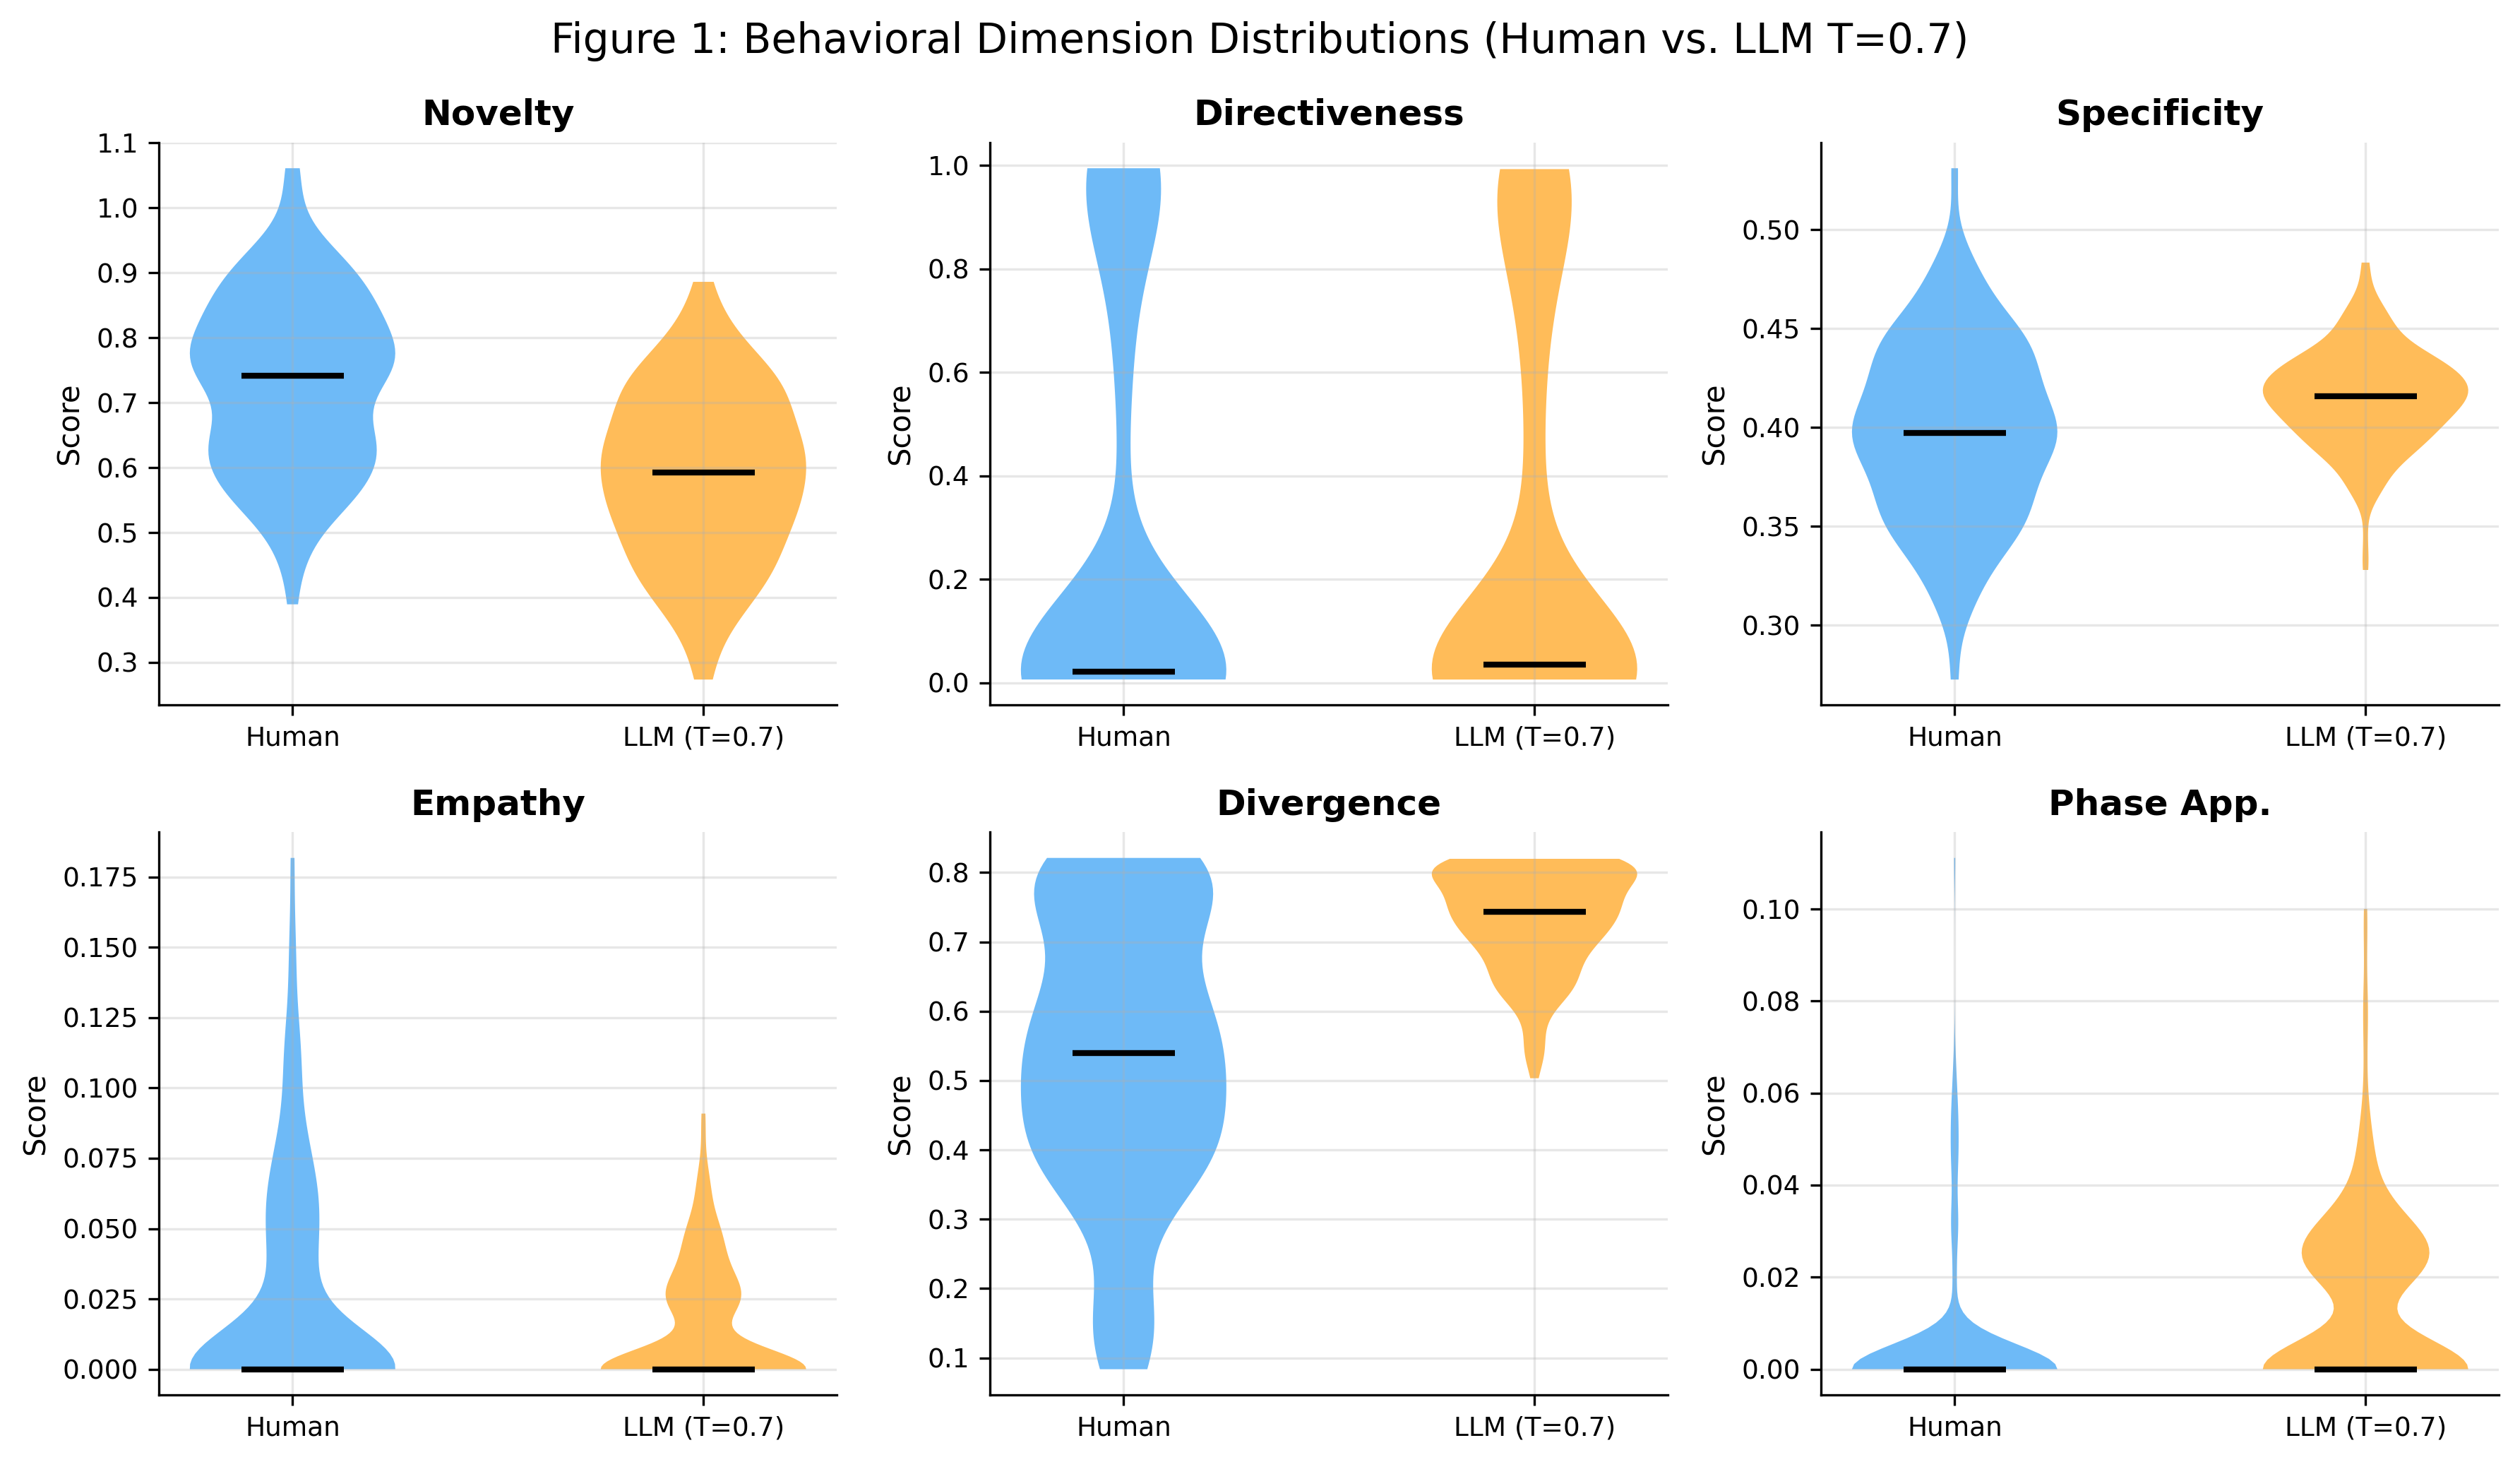
\includegraphics[width=\columnwidth]{figure1_violin_distributions.png}
    \caption{Violin plots showing score distributions for human PM turns and Llama 3.1 8B Instruct ($T=0.7$) responses across the six behavioral dimensions. Horizontal lines indicate medians.}
    \label{fig:distributions}
\end{figure}

PCA projection on standardized features (Fig.~\ref{fig:pca}) showed that PC1 (22.8\% variance) and PC2 (21.3\% variance) together accounted for 44.1\% of variance. Human PM turns clustered toward negative PC1 values, whereas LLM responses shifted toward positive PC1 values with dispersion along PC2.

\begin{figure}[htbp]
    \centering
    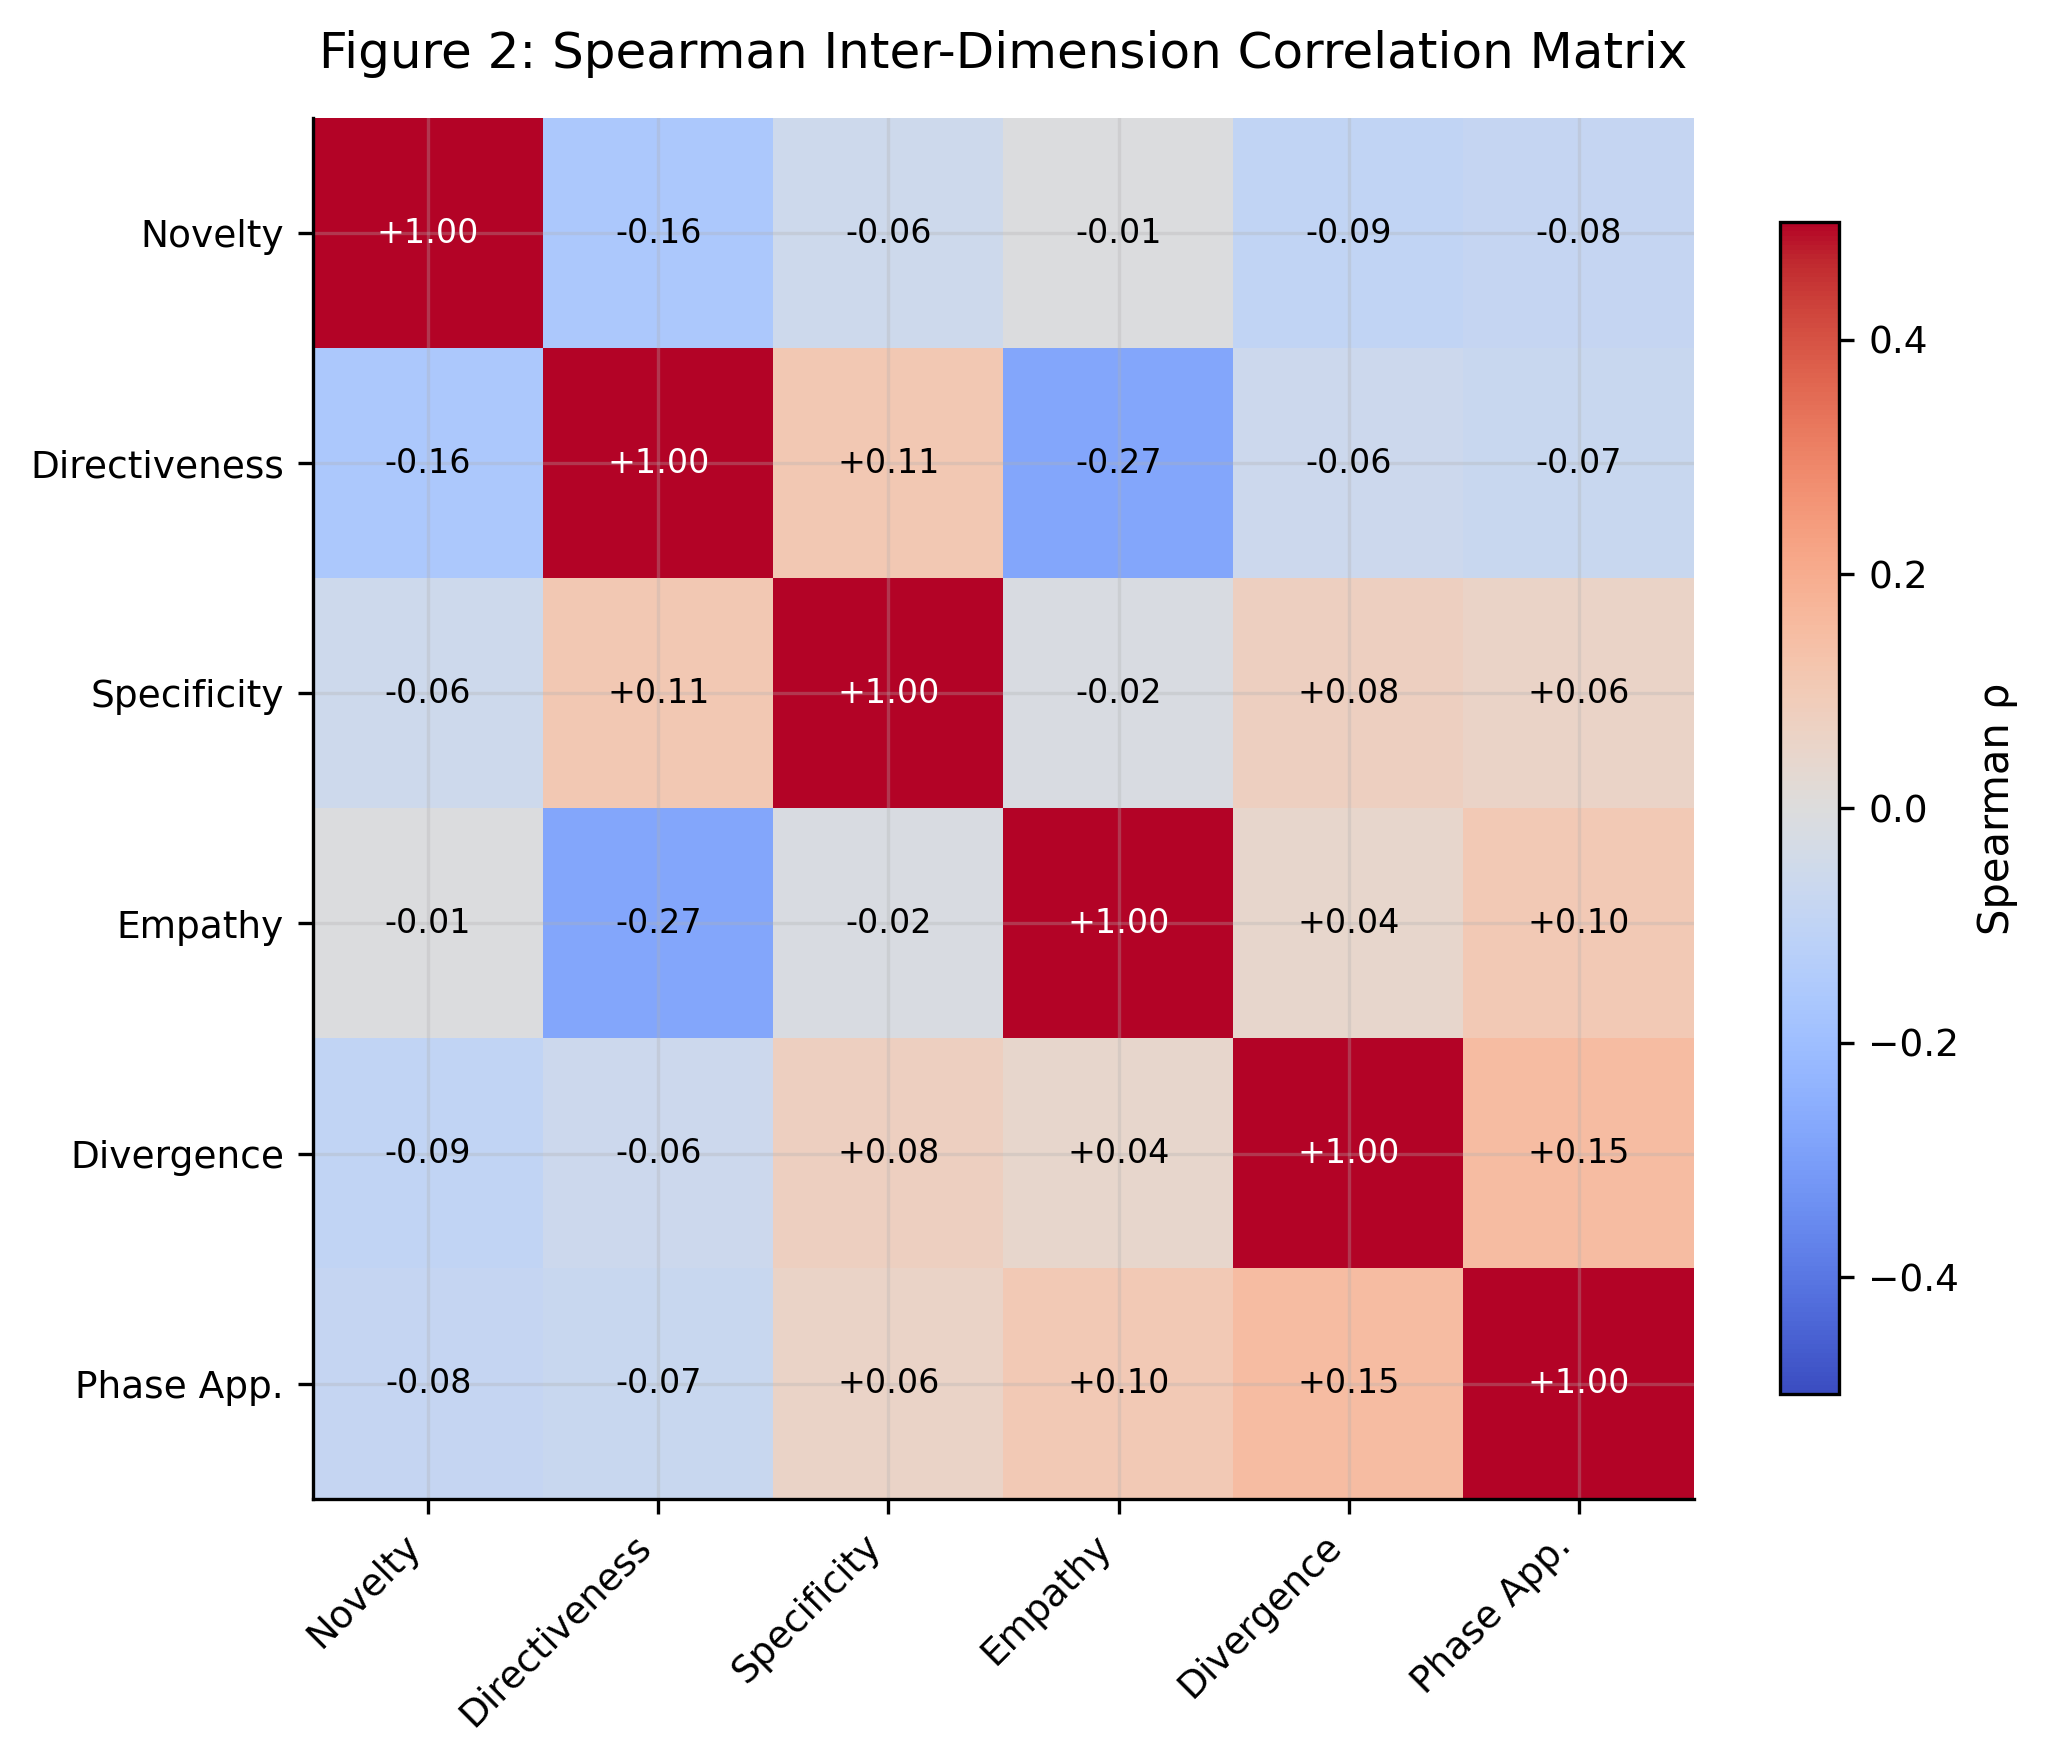
\includegraphics[width=0.85\columnwidth]{figure2_correlation_matrix.png}
    \caption{Spearman correlation matrix across the six behavioral dimensions ($N = 796$). Pairwise correlations remain weak ($|\rho| < 0.28$).}
    \label{fig:corrmatrix}
\end{figure}

\begin{figure}[htbp]
    \centering
    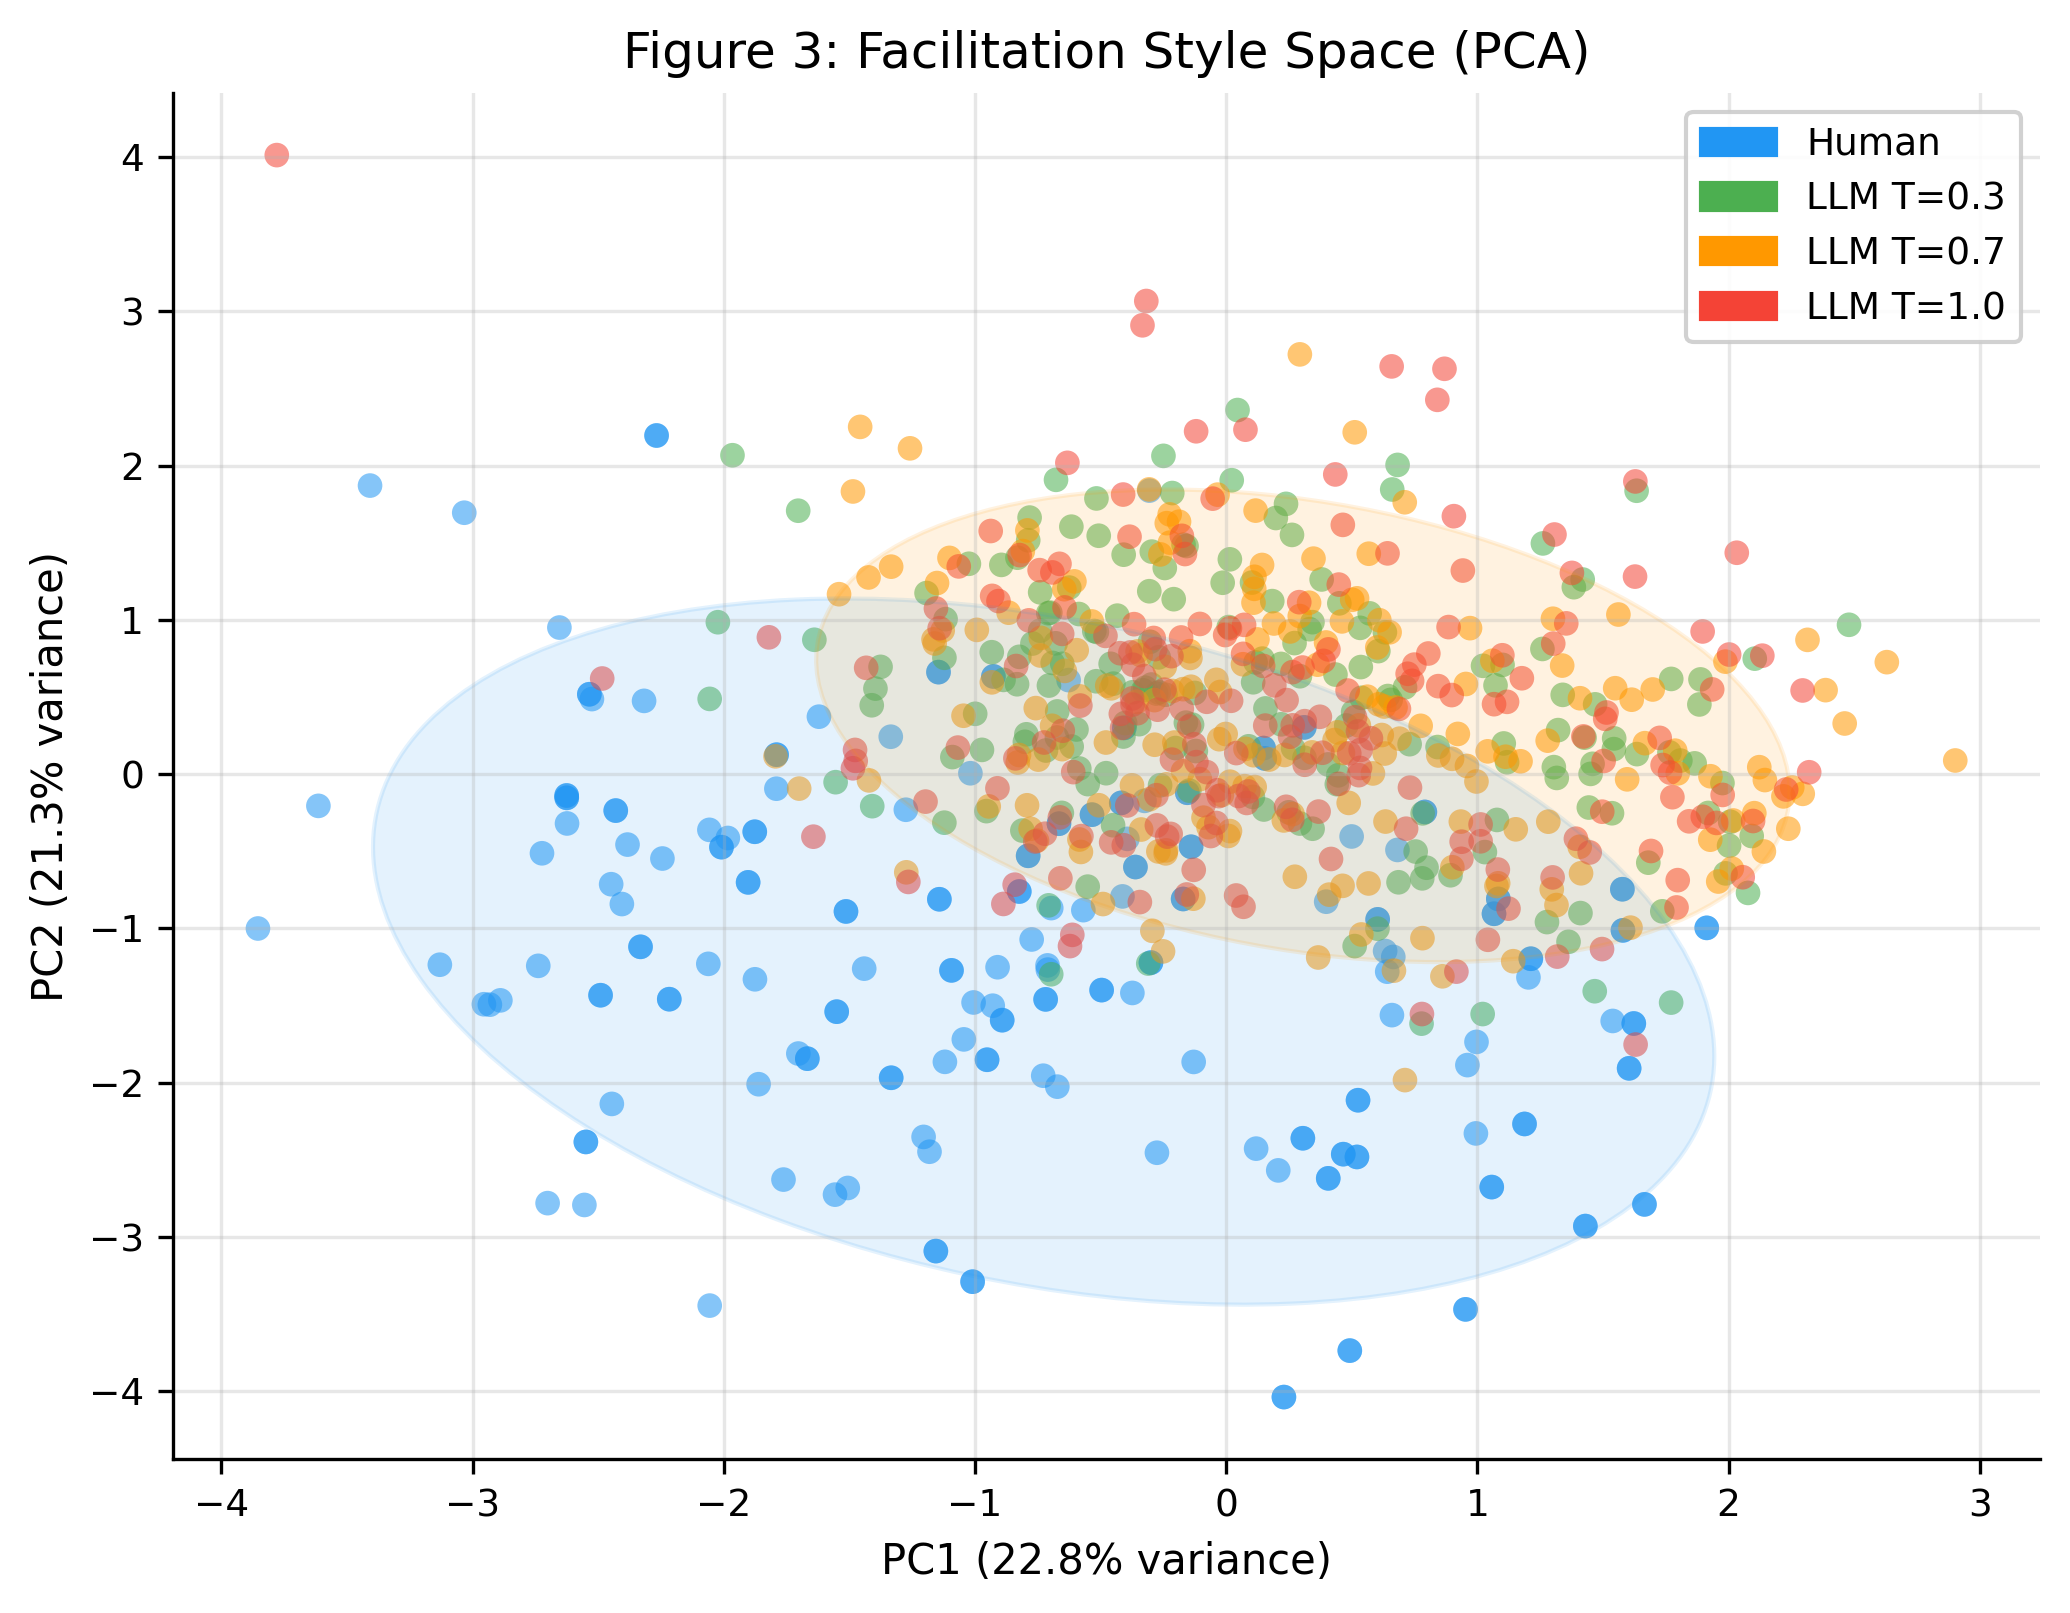
\includegraphics[width=\columnwidth]{figure3_pca_biplot.png}
    \caption{Principal Component Analysis (PCA) projection of the behavioral feature space.}
    \label{fig:pca}
\end{figure}

Spearman correlation analysis across LLM temperatures ($0.3, 0.7, 1.0$; $N=597$) indicated that feature scores were largely temperature-stable (Table~\ref{tab:temp}). Weak significant correlations were observed for specificity ($\rho = +0.116$, $p = 0.005$) and phase alignment ($\rho = -0.102$, $p = 0.013$).

\begin{table}[htbp]
\caption{Spearman correlations between decoding temperature and feature scores ($N = 597$).}
\label{tab:temp}
\centering
\small
\begin{tabular}{@{}lccc@{}}
\toprule
\textbf{Dimension} & \textbf{$\rho$} & \textbf{$p$} & \textbf{Sig.} \\
\midrule
Contextual Distance & $-$0.012 & 0.772 & --- \\
Directiveness (Exp.) & $-$0.010 & 0.804 & --- \\
Specificity Proxy   & +0.116   & 0.005 & ** \\
Empathy Lexicon     & +0.005   & 0.903 & --- \\
Topic Divergence    & $-$0.056 & 0.170 & --- \\
Phase Alignment     & $-$0.102 & 0.013 & * \\
\bottomrule
\end{tabular}
\end{table}

\begin{figure}[htbp]
    \centering
    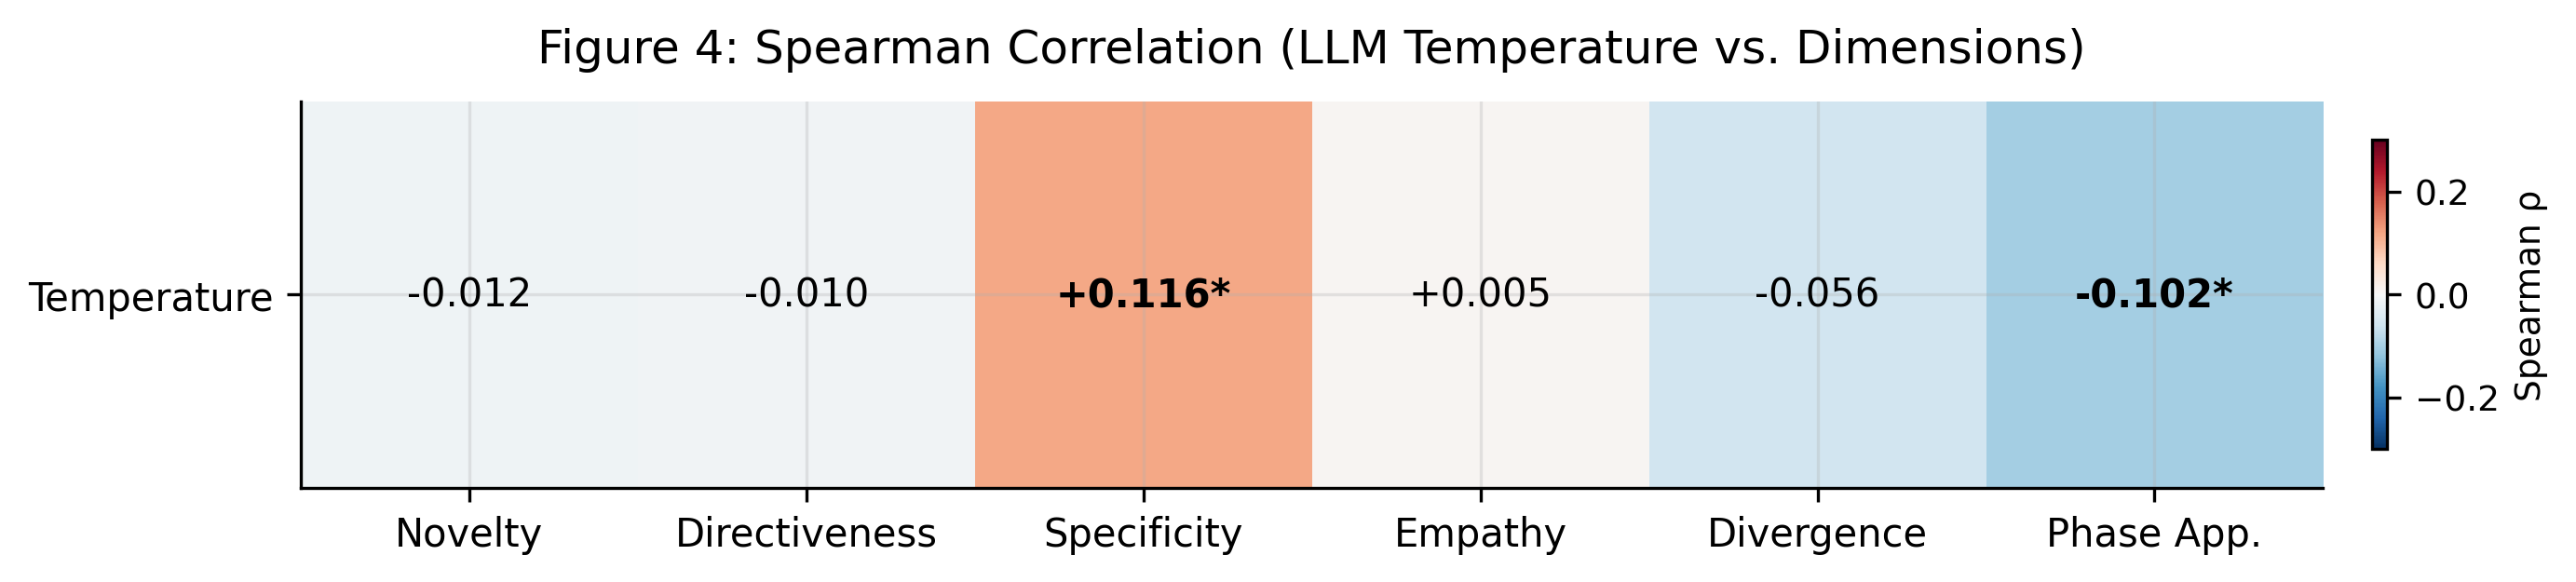
\includegraphics[width=\columnwidth]{figure4_temperature_heatmap.png}
    \caption{Heatmap of median feature scores across human PM turns and LLM temperatures.}
    \label{fig:heatmap}
\end{figure}

\begin{figure}[htbp]
    \centering
    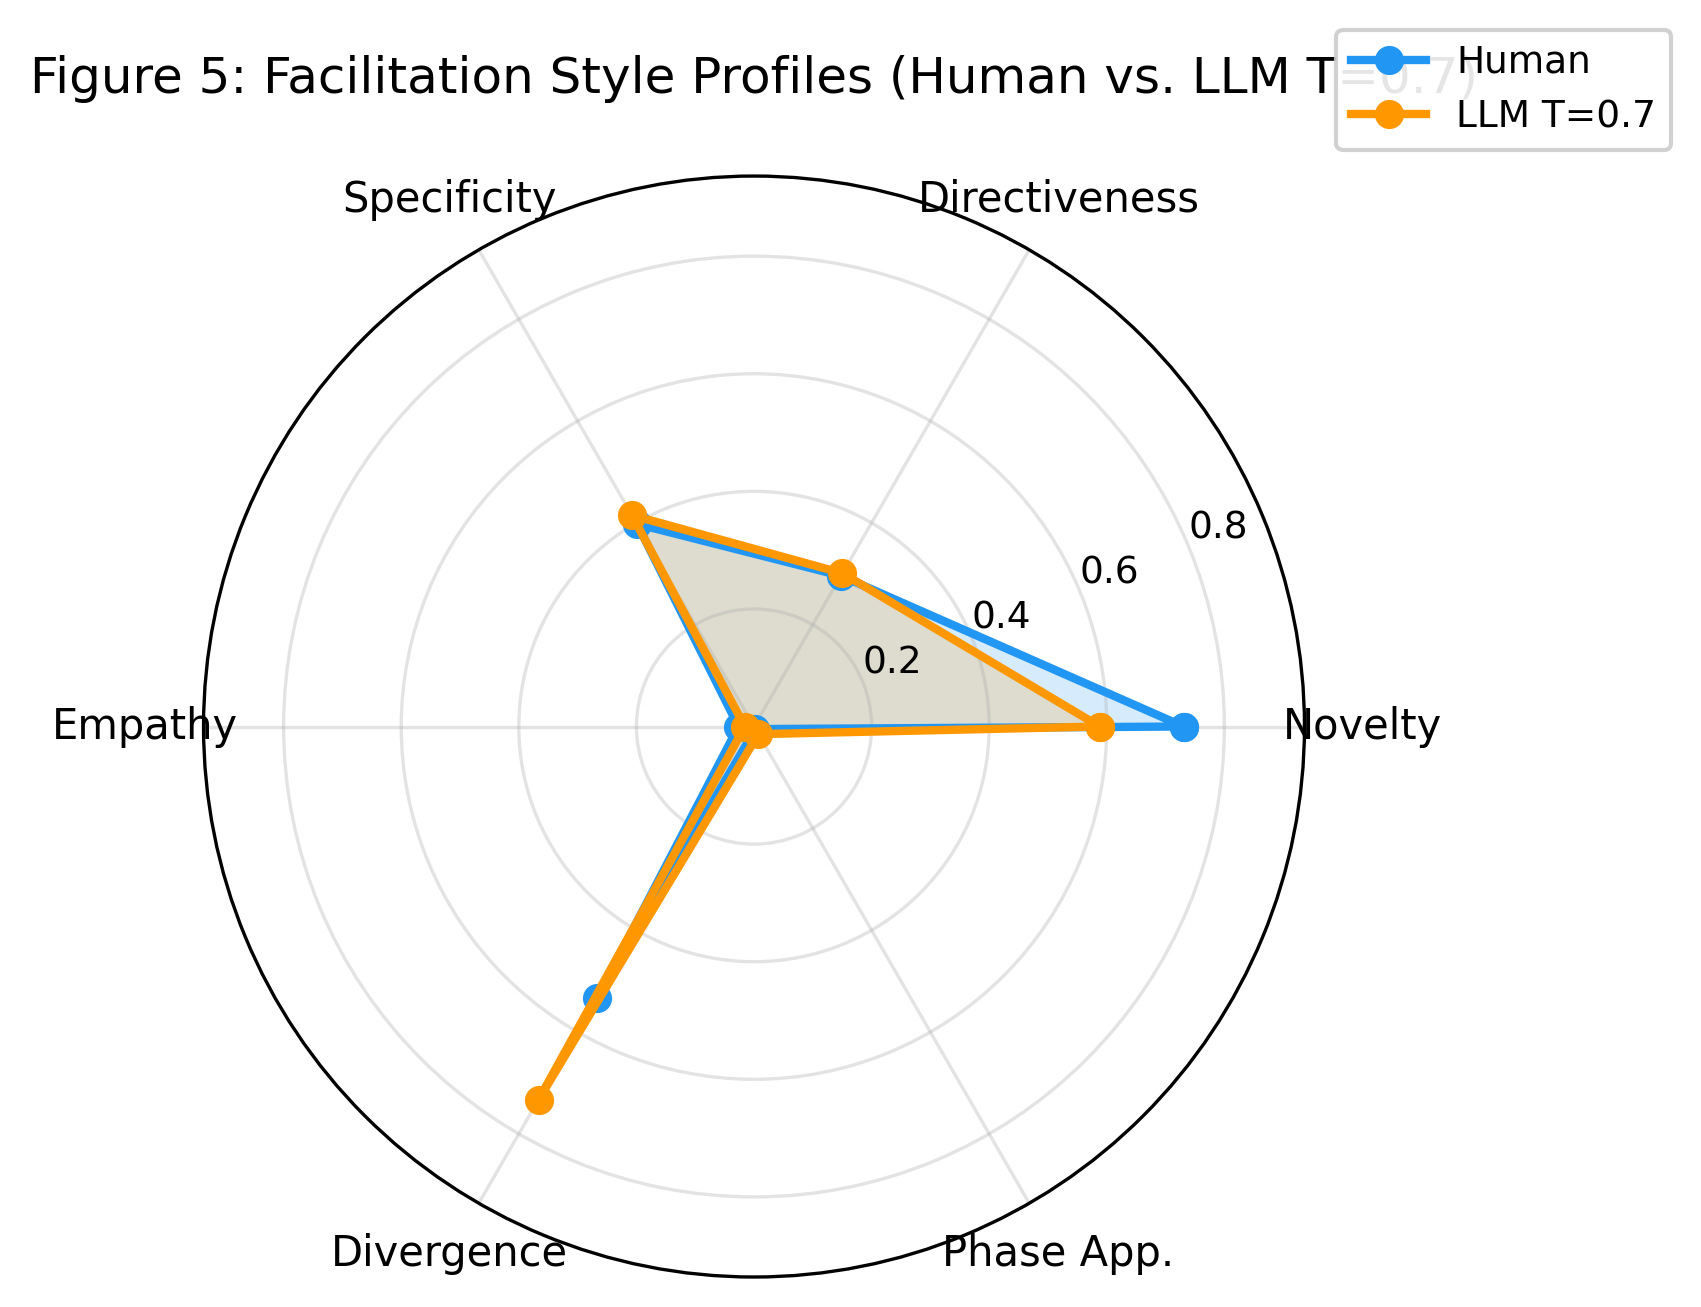
\includegraphics[width=0.85\columnwidth]{figure5_radar_profiles.png}
    \caption{Radar chart comparing median behavioral profiles of human PM turns and LLM responses.}
    \label{fig:radar}
\end{figure}

Sensitivity analyses evaluating response length and session clustering remained qualitatively consistent with primary findings (Table~\ref{tab:robustness}). In length-matched subsampling ($n = 72$), differences remained significant for contextual distance ($r = -0.309$), topic divergence ($r = +0.499$), specificity proxy ($r = +0.706$), and phase alignment ($r = +0.281$). Partial Spearman correlations and linear mixed-effects models (`statsmodels` MixedLM) confirmed these directions.

\section{Discussion}
The empirical comparison indicates distinct output properties between Llama~3.1 8B Instruct responses and human Project Manager turns in the AMI design scenario. Higher topic divergence ($r = +0.580$) in LLM responses indicates that generated moves introduce thematic content further from the immediate 5-turn context in LDA topic space. Human PM turns displayed higher embedding-space contextual distance ($r = -0.537$), reflecting distinct phrasing while remaining topic-bound.

Several limitations constrain interpretation:
(1)~Evaluation was conducted exclusively on Llama~3.1 8B Instruct (4-bit quantized).
(2)~Human turns were drawn from Project Manager participants in the AMI remote-control design scenario, which may not represent professional design facilitators in industry settings.
(3)~The DistilBERT directiveness classifier achieved high accuracy on synthetic test data but failed human validation on 100 AMI utterances ($\kappa = -0.0231$). Directiveness results are exploratory and unvalidated.
(4)~Design phase labels were explicitly provided in the LLM prompt, and phase assigned by temporal position.
(5)~Specificity and empathy measures rely on surface lexical proxies.
(6)~Non-significant findings for directiveness ($p_{\text{Bonf}} = 1.000$, power = 0.05) and empathy ($p_{\text{Bonf}} = 1.000$, power = 0.21) reflect insufficient power and cannot demonstrate equivalence.
(7)~Independent-Sample Inferential Assumption: The 199 LLM responses at each temperature are context-matched to the 199 human PM turns, and the three temperatures reuse the same 199 contexts. However, the primary inferential analyses utilize independent-sample Mann-Whitney $U$ tests. The tests do not model paired or hierarchical error structures and should be interpreted as independent-sample comparisons rather than fully paired hierarchical inference.

\section{Conclusion}
This study compared Llama~3.1 8B Instruct responses with naturally occurring human Project Manager turns from the AMI Meeting Corpus across six computational behavioral dimensions. Statistically significant differences were observed on four dimensions: Llama~3.1 8B Instruct generated responses with higher topic divergence ($r = +0.58$), higher specificity proxy ($r = +0.25$), and higher phase-vocabulary alignment ($r = +0.34$), whereas human PM turns exhibited greater contextual semantic distance ($r = -0.54$). Directiveness and empathy showed no significant differences under low statistical power. These results document baseline behavioral characteristics of Llama~3.1 8B Instruct in meeting facilitation contexts and highlight methodological considerations for computational facilitation research.

\section*{Declaration of Interest}
The authors declare no conflict of interest.

\section*{Data Availability}
The AMI Meeting Corpus is available at \url{https://groups.inf.ed.ac.uk/ami/corpus/}. Code and data are available at \url{https://github.com/Ayaan577/llm-facilitation-behavior}.

\bibliographystyle{IEEEtran}
\bibliography{main_chb}

\appendices
\section{Robustness Check Results}
\label{app:robustness}
\begin{table}[h]
\caption{Robustness Checks---Length-Matched Subsampling, Partial Correlations, and MixedLM Results (Human PM vs.\ LLM $T=0.7$).}
\label{tab:robustness}
\centering
\small
\begin{tabular}{lcccccc}
\toprule
\textbf{Dimension} & \textbf{Orig $r$} & \textbf{Match $r$} & \textbf{Part $\rho$} & \textbf{ME $\beta$} & \textbf{$p_{\text{Bonf}}$} & \textbf{Stability} \\
\midrule
Contextual Distance  & $-$0.54 & $-$0.31 & $-$0.23 & $-$0.143 & $<$0.001 & Stable \\
Topic Divergence     & +0.58   & +0.50   & +0.41   & +0.199   & $<$0.001 & Stable \\
Specificity Proxy    & +0.25   & +0.71   & +0.51   & +0.017   & $<$0.001 & Stable \\
Phase Alignment      & +0.34   & +0.28   & +0.18   & +0.010   & $<$0.001 & Stable \\
Empathy Lexicon      & $-$0.06 & $-$0.15 & $-$0.20 & $-$0.011 & 0.005    & Mixed  \\
Directiveness (Exp.) & $-$0.005 & $-$0.18 & $-$0.11 & +0.005  & 1.000    & Unvalidated \\
\bottomrule
\end{tabular}
\end{table}

\end{document}
